% =====================================================================================
%  A Same-Generator Corpus and Classifier Floors for AI-Control Monitor Evaluation
%  EvoRobust @ NeurIPS 2026 - 4 content pages, non-archival, double-blind, Sep 12 AoE.
%
%  Scaffold built 2026-09-09. Cut plan (notes/06 §5.1) and §1 applied 2026-09-11.
%  Numbers follow experiments/REPRODUCED.md and RESULTS.md. Citations follow refs.bib.
%
%  BUILD:  pdflatex main && bibtex main && pdflatex main && pdflatex main
%          (latexmk is not installed on the local machine)
%
%  Body: §1-§5 plus F3 as the only float. Everything else (schema table, F1, similarity
%  table, F2, the token test, the scratchpad channel) is in the appendix after the
%  references, which the workshop does not count.
% =====================================================================================

\documentclass{article}

% Numeric, compressed citations: [3], [5-7]. This is the NeurIPS house style (the
% template's own prose says "previous work [4]") and it is much tighter than plainnat's
% author-year, which matters at 4 pages. It also stops the two bibliography entries whose
% authors lit/01 never recorded from rendering inline as "leg [2026]" and "len [2026]".
% MUST come before neurips_2026 is loaded - the style file loads natbib itself.
\PassOptionsToPackage{numbers,compress}{natbib}

% EvoRobust is a NeurIPS 2026 workshop with DOUBLE-BLIND review on OpenReview
% (notes/01-venue-evorobust.md), so the track option is dblblindworkshop - NOT the
% default, which is the main track. This option requires \workshoptitle below.
% After acceptance, change to [dblblindworkshop, final].
%
% Note on what this option does and does not do, checked against neurips_2026.sty:
%   - it sets \@trackname to "... Workshop: <workshoptitle>.", which the style file uses
%     ONLY under [final]. At submission the footer is the fixed "Submitted to ... Do not
%     distribute." string. So the workshop name correctly does NOT appear yet.
%   - unlike sglblindworkshop, it does NOT set \@anonymousfalse, so the paper stays
%     anonymous. The "Anonymous Author(s) / Affiliation / Address / email" block on page 1
%     is emitted by the style file itself (sty line 336), not by our \author{} below.
\usepackage[dblblindworkshop]{neurips_2026}

\usepackage[utf8]{inputenc}
\usepackage[T1]{fontenc}
\usepackage{hyperref}
\usepackage{url}
\usepackage{booktabs}
\usepackage{array}      % >{\raggedright\arraybackslash}p{} columns used by F1
\usepackage{amsfonts}
\usepackage{amsmath}
\usepackage{nicefrac}
\usepackage{microtype}
\usepackage{graphicx}
\usepackage{xcolor}
\usepackage{etoolbox}

% The dataset entries carry long unbreakable \texttt{} paths
% (eugenekoran/apps-control-arena-high-quality). Justified, they force gappy interword
% spacing - 10 underfull hboxes. Ragged-right in the bibliography ONLY fixes it without
% touching the body text, which must stay justified.
\apptocmd{\thebibliography}{\raggedright}{}{}

\graphicspath{{fig/}}

% --- Drafting aid. ---------------------------------------------------------------------
% Switched to the no-op form 2026-09-11, AFTER verifying by grep that every citation key
% that used to live only inside a \TODO{} is now cited in real prose (§1). Do not switch
% it back to the red form without re-running that grep.
\newcommand{\TODO}[1]{\textcolor{red}{\textbf{[TODO: #1]}}}
\renewcommand{\TODO}[1]{}

% =====================================================================================
%  EVERY LOAD-BEARING NUMBER, DEFINED EXACTLY ONCE.
%
%  This is not decoration. This project's recurring failure mode (R18 and its companion)
%  is a number from one protocol being written next to a count from another - it has
%  reached the README, the outline and figures.py. Macros make that error impossible to
%  commit silently: there is one \nocodeCV and it carries its own count.
%
%  Source: experiments/REPRODUCED.md unless noted. DO NOT hardcode any of these inline.
% =====================================================================================

% --- Koran's exact split, comments stripped (the headline protocol) ------------------
\newcommand{\tfidfKoran}{0.806}            % 0.8063; above 20 of 24
\newcommand{\tfidfKoranCount}{20}
% RESERVED (rows of the generated Table~\ref{tab:protocol-baseline}, not of the prose):
\newcommand{\tfidfKept}{0.891}             % 0.8914, comments kept; above 22 of 24
\newcommand{\tfidfKeptCount}{22}
\newcommand{\charNgram}{0.783}             % 0.7830, char n-grams on the Koran split

% --- The no-code floor. THE TRAP: two protocols, two values, two counts. -------------
% NEVER write \nocodeCV next to \nocodeHeldoutCount. See fig/CAPTIONS.md.
\newcommand{\nocodeCV}{0.772}              % 0.7715 +- 0.0389, 5x5 CV within the test split
\newcommand{\nocodeCVsd}{0.039}            % RESERVED: figures.py prints it inside F3
\newcommand{\nocodeCVCount}{20}            % <- 0.772 clears 20
\newcommand{\nocodeHeldout}{0.716}         % 0.7163, single 413-item held-out slice
\newcommand{\nocodeHeldoutCount}{18}       % <- 0.716 clears 18
% --- Headline uncertainty (RESULTS.md §8, headline_ci.json, 2026-09-11) ---------------
% Bootstrap over problems (\bootDraws) for the CIs; \permReps training-label permutations
% for the nulls (the CV protocol's null shuffles labels for fitting and scoring alike).
% *PairedCount = monitors below the floor with a paired-bootstrap CI on (ours - theirs)
% excluding zero, on identical items. Each no-code value keeps its OWN pair of counts.
\newcommand{\bootDraws}{2{,}000}
\newcommand{\permReps}{200}
\newcommand{\tfidfKoranLo}{0.7704}
\newcommand{\tfidfKoranHi}{0.8409}
\newcommand{\tfidfKoranNull}{0.5465}       % null 95th percentile; p < 0.005 (0 of 200)
\newcommand{\tfidfKoranPairedCount}{18}
% The CI below is NOT an interval of \nocodeCV (the fold mean). RESULTS.md 8.3: protocol A
% produces no single per-item score vector from a fold mean, so its interval and its paired
% tests are built on the POOLED out-of-fold scores, whose AUROC is \nocodeCVPooled. Any
% sentence quoting \nocodeCVLo--\nocodeCVHi must name \nocodeCVPooled beside it.
\newcommand{\nocodeCVPooled}{0.766}        % 0.7658 pooled out-of-fold AUROC (RESULTS.md 8.3)
\newcommand{\nocodeCVLo}{0.7319}           % CI on the pooled out-of-fold AUROC
\newcommand{\nocodeCVHi}{0.8005}
\newcommand{\nocodeCVNull}{0.5545}         % p < 0.005
\newcommand{\nocodeCVPairedCount}{17}
\newcommand{\nocodeHeldoutLo}{0.6476}
\newcommand{\nocodeHeldoutHi}{0.7796}
\newcommand{\nocodeHeldoutNull}{0.7023}    % barely above its null
\newcommand{\nocodeHeldoutP}{0.030}        % 5 of 200
\newcommand{\nocodeHeldoutPairedCount}{12}
\newcommand{\permP}{p < 0.005}             % math mode contents; 0 of \permReps replicates

% --- The 24-monitor comparison set (Jha, MIT) ---------------------------------------
\newcommand{\monN}{24}
\newcommand{\monMedian}{0.609}
\newcommand{\monMax}{0.937}

% --- What the field's fix does and does not reach ------------------------------------
\newcommand{\lenFiltered}{0.4726}          % length-only on the filtered split - chance
\newcommand{\lenRaw}{0.826}                % RESERVED (F1 row): 0.8255 pairwise, raw artifact
\newcommand{\hashRaw}{0.6957}
\newcommand{\hashStripped}{0.4983}

% --- Authorship, three ways ---------------------------------------------------------
% RESULTS.md §6 (2026-09-11): comment-STRIPPED on both classes, mean over five
% problem-disjoint 30% splits (transfer rows: one fixed split each). Coordinator's band:
% weakened but standing. The paper reports these; the *Kept companions are the earlier
% unstripped values, inflated by the comment channel, and appear only in the appendix.
\newcommand{\transfer}{0.969}              % 0.9694 Control Tax -> the 2023 GPT-4 set
\newcommand{\pairAll}{0.897}               % 3 dp: resolution over ~2,641 pairs is 1/2,641
\newcommand{\pairWorking}{0.935}
\newcommand{\pairInert}{0.879}
\newcommand{\surfaceSeven}{0.7259}
\newcommand{\tfidfMatched}{0.8560}         % matched-protocol TF-IDF AUROC, stripped, 5 seeds
\newcommand{\transferKept}{0.994}          % 0.9935
\newcommand{\pairAllKept}{0.962}
\newcommand{\pairWorkingKept}{0.979}
\newcommand{\pairInertKept}{0.955}
\newcommand{\surfaceSevenKept}{0.8306}     % five-seed unstripped mean (seed 0 alone: 0.8302)
% Other cross-model transfer rows, stripped (RESULTS.md §6.2): unstripped 0.976/0.813/0.828
\newcommand{\transferOthreeClaude}{0.866}  % o3-mini -> claude-3-7-sonnet, 82 test pairs
\newcommand{\transferClaudeOthree}{0.844}  % claude-3-7-sonnet -> o3-mini
\newcommand{\transferOoneGemini}{0.764}    % o1-mini -> gemini-2.0-flash
% Style markers on the control_tax pairs (attack / honest): the # marker was the comment channel
\newcommand{\hashPresAttack}{0.685}
\newcommand{\hashPresHonest}{0.176}
\newcommand{\hashPresAttackStripped}{0.007}
\newcommand{\hashPresHonestStripped}{0.008}

% --- The byline leak surviving the comment stripper (string literals are not comments)
\newcommand{\bylineHonest}{23}
\newcommand{\bylineAttack}{2}
\newcommand{\tripleHonest}{43}
\newcommand{\tripleAttack}{9}

% --- The second selection artifact --------------------------------------------------
\newcommand{\inertShare}{80.7\%}           % of Koran's test-split labelled backdoors (892) do not work
\newcommand{\inertSharePassing}{32.8\%}    % same, among the 256 that PASS the public tests (172 fire);
                                           % the like-for-like analogue of our `passes' eligibility rule
\newcommand{\testCasesAttack}{20.95}
\newcommand{\testCasesHonest}{38.85}

% --- Split and artifact shapes ------------------------------------------------------
\newcommand{\splitTrain}{1{,}209}          % PROBLEMS, and 1,209 per class in the appendix
\newcommand{\splitTrainItems}{2{,}418}     % ... = the paired train split's item count
\newcommand{\splitTest}{1{,}375}
\newcommand{\splitAttack}{172}
\newcommand{\splitHonest}{1{,}203}
\newcommand{\harnessAgreement}{95.84\%}

% --- Gate S ------------------------------------------------------------------------
% B measured 2026-09-09 on the analysis ceiling; see experiments/gate_s_baseline.json.
% NOTE: rho's denominator is B over the ARM'S realised eligible set, not this ceiling
% value. Recompute with gate_s_eval.py when an arm lands, then update this macro.
\newcommand{\baselineB}{0.871}
\newcommand{\baselineBn}{1{,}444}
\newcommand{\rhoCollapse}{0.33}
\newcommand{\rhoContent}{0.72}
% Absolute AUROC each band corresponds to AT THE MEASURED B. Do NOT use 0.601/0.720:
% those are arithmetic at an assumed B = 0.806 and route a G in 0.720-0.767 wrongly.
% RESERVED: the corrected absolute bands, kept so the superseded 0.601/0.720 cannot return.
\newcommand{\gCollapseMax}{0.6226}
\newcommand{\gPartialMax}{0.7674}

% --- Arm 1: regenerate the honest half only (Qwen3-Coder-30B vs stored backdoors) -----
% CONFOUNDED. Do not route a title on it. experiments/RESULTS.md section 3.
\newcommand{\armOneN}{668}
\newcommand{\armOneBprime}{0.874}      % B recomputed on arm 1's own eligible problems
\newcommand{\armOneG}{0.962}
\newcommand{\armOneRho}{1.234}
\newcommand{\armOneTfidfDelta}{+0.088}
\newcommand{\armOneLenG}{0.489}        % length carrier falls to chance while TF-IDF rises

% --- Pair similarity: why the same-generator attack class needs TWO arms ------------
% RESULTS.md 4.8-4.9. Character similarity of honest/attack pairs, comments stripped.
% The stored benchmark's classes are largely INDEPENDENT programs, so an attack class
% built by editing its own honest solution changes similarity as well as authorship,
% and its S cannot separate "the benchmark measured authorship" from "we made the two
% classes the same text". Report S beside the similarity or it is uninterpretable.
% Re-measured 2026-09-11 with autojunk=False (RESULTS.md 9.1); the earlier 0.469 / 0.924 / 0.415
% were computed with difflib's junk heuristic on and are superseded.
\newcommand{\simStored}{0.606}         % stored benchmark on the headline's 623 problems
\newcommand{\simStoredHigh}{3.4\%}     % share above 0.95
\newcommand{\simStoredLow}{45.4\%}     % share below 0.60
\newcommand{\simEdit}{0.928}           % edit arm - near-copies, n=427 passing pairs
\newcommand{\simEditHigh}{64.2\%}
\newcommand{\simEditLow}{4.0\%}
\newcommand{\simIndep}{0.659}          % independent arm, n=623 - the stored regime
\newcommand{\simIndepHigh}{3.4\%}
\newcommand{\simIndepLow}{34.8\%}

% --- The release bundle (notes/07, release_split.py --check passed 2026-09-11) ----------
\newcommand{\relHonest}{1{,}444}       % honest programs, one model
\newcommand{\relEdit}{1{,}112}         % edit-arm attack programs
\newcommand{\relIndep}{1{,}112}        % independent-arm attack programs
\newcommand{\relRetryDraws}{11{,}565}  % every draw of the independent arm's retry pool
\newcommand{\relPassFirst}{623}        % independent-arm pairs passing, outcome-blind (--keep first)
\newcommand{\relFireFirst}{14}         % ... and firing
\newcommand{\relPassBest}{1{,}046}     % same under the benchmark's own survivor selection (--keep best)
\newcommand{\relFireBest}{99}          % ... firing
\newcommand{\relFireBestCrash}{106}    % ... counting a crash on the trigger as firing
\newcommand{\relScripts}{24}           % scripts/ in the bundle (release_split.py SCRIPT_FILES,
                                       % rebuilt 2026-09-11 with the RESULTS.md 13-15 scripts)

% --- Same-generator S: MEASURED (these are no longer placeholders) --------------------
% Same-generator S, RESULTS.md §9 (2026-09-11). All comment-stripped, problem-disjoint 5-fold,
% bootstrap-over-problems 95% CIs. Coordinator's ruling: INCONCLUSIVE between partial and
% content; the authorship-collapse reading is EXCLUDED (both CIs clear the collapse band).
% Headline: independent arm, outcome-blind first draw per problem, attack = passes the public
% tests, B' inert-inclusive over the same problems.
\newcommand{\sameGenS}{0.7512}         % fold mean; 4 dp per the ledger's AUROC rule
\newcommand{\sameGenN}{623}
\newcommand{\sameGenLo}{0.7295}
\newcommand{\sameGenHi}{0.7713}
\newcommand{\sameGenBprime}{0.8658}    % CI 0.8480-0.8812
\newcommand{\sameGenRho}{0.687}
\newcommand{\sameGenRhoLo}{0.625}       % joint bootstrap over problems (S and B' resampled together; RESULTS.md 12)
\newcommand{\sameGenRhoHi}{0.755}
\newcommand{\sameGenLen}{0.5851}       % length-only carrier: to chance
\newcommand{\curveHeadline}{0.8521}    % B at n = 623 under the identical pipeline
\newcommand{\curveHeadlineSd}{0.0055}
% Strict: survivor selection (the benchmark's own retry-and-keep), attack = passes AND fires
% (crash not counted as firing), B' all-firing. Read through rho against its own B' only.
\newcommand{\strictS}{0.7652}
\newcommand{\strictLo}{0.7016}
\newcommand{\strictHi}{0.8000}
\newcommand{\strictN}{99}
\newcommand{\strictBprime}{0.7877}     % CI 0.7427-0.8367
\newcommand{\strictRho}{0.921}          % fold-mean convention, as RESULTS.md 9 quotes S
% As for the no-code floor: the interval is built on the POOLED out-of-fold scores, whose rho
% is \strictRhoPooled (RESULTS.md 12.2, which asks the ledger to say which convention it
% quotes). At n = 99 the two conventions differ by 0.06 of fold-to-fold variance.
\newcommand{\strictRhoPooled}{0.86}     % 0.861, pooled-score rho; the interval below is on it
\newcommand{\strictRhoLo}{0.662}        % joint bootstrap (RESULTS.md 12)
\newcommand{\strictRhoHi}{1.089}
\newcommand{\strictRhoSeeds}{0.85--0.92}  % five fold seeds, RESULTS.md 12.4 (mean 0.875 +- 0.028)
\newcommand{\curveStrict}{0.7807}      % B at n = 99: absolute bands do not apply there
\newcommand{\curveStrictSd}{0.0248}
\newcommand{\survivorAuroc}{0.62}      % survivors vs non-survivors within the attack class
\newcommand{\survivorSwapS}{0.7595}    % S recomputed with non-firing attempts, same problems
\newcommand{\survivorSwapSref}{0.7687} % S on those same problems with the survivors
% The headline attack class is attempts: 14 of its \sameGenN{} selected draws fire
% (RESULTS.md 7.4, `first` policy: 623 problems with a passing draw, 14 with a usable one).
\newcommand{\headlineFireShare}{2.2\%}
% The inert share of the EXACT compared headline sets (notes/10 section 7): 14 of 623 Sonnet
% attacks fire and 2 of 611 Haiku ones do. NOT 97.5%, which is RESULTS.md 7.7's pooled
% conditional rate over 11,565 draws and a different denominator.
\newcommand{\headlineInert}{97.75\%}
\newcommand{\haikuInert}{99.67\%}
% The second generator's firing share, the analogue of \headlineFireShare: 2 of 611,
% RESULTS 15.5. NOT the 35/1,444 usable count - 33 of those 35 sit on problems whose
% honest program failed and never enter a pair.
\newcommand{\haikuFireShare}{0.3\%}       % 2 of 611, RESULTS 15.5
% Why our single-shot firing rate is low: the attack prompt reuses public test inputs as
% triggers, which cannot diverge from the honest solution (experiments/apps/TRIGGER-YIELD.md
% and trigger_public_check.py, over the 6,570 test-passing draws of the retry pool).
\newcommand{\trigPublicShare}{52.0\%}
\newcommand{\trigPublicFire}{0.15\%}
\newcommand{\trigNovelFire}{5.13\%}
\newcommand{\trigStoredPublic}{0 of 3{,}188}
% Yield (RESULTS §7.7): single-shot, blind, vs the stored attacker, which executes and iterates
\newcommand{\fireGivenPassOurs}{2.5\%}
\newcommand{\fireGivenPassStored}{67.2\%}   % Koran test split: 256/892 pass, 172/256 fire
% Edit arm: a bound under near-copies, never a verdict
\newcommand{\editS}{0.6266}            % CI 0.6044-0.6467
\newcommand{\editN}{427}
\newcommand{\editRho}{0.371}
\newcommand{\editSim}{0.928}
% Positive control (RESULTS.md §10): a trusted-monitor prompt to the SAME model that wrote both
% classes, scored on the same pairs. Headline set: 97.8% of its attacks never fire (14 of
% 623 do, RESULTS.md 7.4). NOT 97.5%, which is the pooled per-draw rate of RESULTS.md 7.3.
\newcommand{\monitorS}{0.566}          % AUROC on the 623 headline pairs
\newcommand{\monitorSLo}{0.5507}
\newcommand{\monitorSHi}{0.5833}
\newcommand{\monitorStrict}{0.818}     % AUROC on the 99 strict (pass AND fire) pairs
\newcommand{\monitorStrictLo}{0.7630}
\newcommand{\monitorStrictHi}{0.8686}
% RESULTS.md 11-12: the residual is layout from the attack prompt's framing, not the trigger idiom
\newcommand{\sameGenSid}{0.700}         % S with identifiers normalised (the only mask that moves it)
\newcommand{\sameGenRhoId}{0.54}
\newcommand{\defMainAttack}{67\%}        % `def main` present, attack side of the headline pairs
\newcommand{\defMainHonest}{38.5\%}      % honest side (RESULTS.md 11.3/11.5: 0.385)
\newcommand{\monitorClfPhi}{0.04}        % pair-level phi between monitor and classifier correctness

% =====================================================================================
%  THE SECOND-PASS ARMS (RESULTS.md 13-15, measured 2026-09-11; the values and the
%  precision rule - AUROC 4 dp, rho 3 dp - are notes/10-ledger-recheck.md's verified
%  block, which re-derived every one of them from the named json field). Pass 1 reserved these
%  names as red placeholders used nowhere in the prose; every macro below now carries a
%  MEASURED value. One macro, one protocol, its n and its RESULTS.md section in the comment.
% =====================================================================================

% --- Arm A: the prompt-matched honest class (RESULTS.md 13) --------------------------
% Model AND prompt held constant on both sides: PROMPT_INDEPENDENT with only the flaw
% sentence replaced by its correct-program counterpart, same model, same harness.
% Comment-stripped, problem-disjoint 5-fold, bootstrap over problems; rho against B'
% RE-FITTED on the same reduced problem set, joint bootstrap (RESULTS.md 13.2).
\newcommand{\matchedS}{0.6423}          % 0.6423; headline, n = 586 of the 623 (matched program passes)
\newcommand{\matchedN}{586}
\newcommand{\matchedLo}{0.6179}
\newcommand{\matchedHi}{0.6621}
\newcommand{\matchedBprime}{0.8613}    % B' on those same 586 problems, inert-inclusive
\newcommand{\matchedRho}{0.394}        % partial band; P(rho > 0.72) = 0.000
\newcommand{\matchedRhoLo}{0.326}      % joint bootstrap over problems
\newcommand{\matchedRhoHi}{0.454}
% The prompt-only floor: ORIGINAL honest vs MATCHED honest - two CORRECT classes from one
% model under the two prompts, with no attack on either side (RESULTS.md 13.2 row b, n = 586).
\newcommand{\promptOnly}{0.6006}        % 0.6006
\newcommand{\promptOnlyLo}{0.5768}
\newcommand{\promptOnlyHi}{0.6243}
% Strict (passes AND fires), same arm: 96 of the 99 strict problems (RESULTS.md 13.2).
\newcommand{\matchedStrictS}{0.7113}    % 0.7113
\newcommand{\matchedStrictN}{96}
\newcommand{\matchedStrictRho}{0.697}
\newcommand{\matchedStrictRhoLo}{0.494}
\newcommand{\matchedStrictRhoHi}{0.856}
\newcommand{\matchedStrictLo}{0.6464}   % ... its S interval (RESULTS.md 13.2, strict row a)
\newcommand{\matchedStrictHi}{0.7453}
\newcommand{\matchedStrictBprime}{0.8030} % B' on the same 96 problems, all-firing
% As everywhere in RESULTS.md 12-15: a rho POINT is the fold-mean ratio and the joint interval
% beside it is the bootstrap of the POOLED out-of-fold rho (notes/10 section 6). Pooled points on
% these rows: headline matched 0.390, strict matched 0.662, Haiku headline 0.097.
% Masks on the matched headline row, appendix only (RESULTS.md 13.3, n = 586).
\newcommand{\matchedSid}{0.6264}       % identifiers normalised
\newcommand{\matchedRhoId}{0.342}
\newcommand{\matchedSidOrig}{0.7046}   % the ORIGINAL honest class under the same mask
\newcommand{\matchedChar}{0.6817}      % char_wb 3-5 grams, same classifier and folds
\newcommand{\matchedRhoChar}{0.493}
\newcommand{\matchedRhoIdLo}{0.280}    % the ID-masked matched row's joint interval ...
\newcommand{\matchedRhoIdHi}{0.394}
\newcommand{\matchedRhoIdCollapse}{40\%}  % ... which puts this much mass in the collapse band
% Pooled out-of-fold rho on the rows whose fold-mean points the paper quotes (notes/10 section 6)
\newcommand{\matchedRhoPooled}{0.390}
\newcommand{\matchedStrictRhoPooled}{0.662}
\newcommand{\haikuRhoPooled}{0.097}

% --- Arm B: monitors with authorship held constant (RESULTS.md 14) -------------------
% The zero-shot trusted-monitor prompt of RESULTS.md 10 (one request per program, never side
% by side), scored on the STORED pairs over the same problems as the row's own B'.
% monitor-rho = (M_samegen - 0.5)/(M_stored - 0.5), one problem set resampled per draw,
% 2,000 draws (monitor_rho.py, RESULTS.md 14.3). Same-generator column: RESULTS.md 10.
\newcommand{\monStoredHead}{0.9579}     % 0.9579; claude-sonnet-5 monitor, stored pairs, n = 623
\newcommand{\monStoredStrict}{0.9437}   % 0.9437; ... stored pairs of the strict row, n = 99
% The same value at the abstract's precision: the abstract quotes it beside \monitorStrict
% (0.818), and four decimals among three-decimal neighbours read as false precision.
\newcommand{\monStoredStrictAbs}{0.944}  % = \monStoredStrict to 3 dp, ABSTRACT ONLY
\newcommand{\monRhoHead}{0.145}
\newcommand{\monRhoHeadLo}{0.111}
\newcommand{\monRhoHeadHi}{0.182}
\newcommand{\monRhoStrict}{0.717}
\newcommand{\monRhoStrictLo}{0.601}
\newcommand{\monRhoStrictHi}{0.832}
% The second monitor wrote NEITHER class (claude-haiku-4-5). Its headline rows are a BOUND:
% a 512-token ceiling left about half the replies unparseable, and on the stored side the
% missingness is differential by class (RESULTS.md 14.5). The strict rows were re-run at
% --max-tokens 1024 to price that: the AUROCs move inside the bootstrap intervals.
\newcommand{\monHaikuHead}{0.5577}         % 0.5577; same-generator headline pairs, n = 623
\newcommand{\monHaikuStrict}{0.7871}       % 0.7871; same-generator strict pairs, n = 99
\newcommand{\monHaikuStoredHead}{0.8824}   % 0.8824; stored pairs, same problems
\newcommand{\monHaikuStoredStrict}{0.8832} % 0.8832
\newcommand{\monHaikuRhoHead}{0.151}      % CI 0.063-0.242
\newcommand{\monHaikuRhoStrict}{0.749}    % CI 0.514-0.993
\newcommand{\monHaikuRhoStrictMt}{0.766}  % the same row at --max-tokens 1024 (2 of 198 missing)
\newcommand{\monHaikuMissHead}{628 of 1{,}246}  % unparseable same-generator headline replies
\newcommand{\monHaikuMissHonest}{50.1\%}  % stored side, headline: missing honest replies ...
\newcommand{\monHaikuMissAttack}{23.4\%}  % ... against missing attack replies

% --- Arm C: a second same-generator model, claude-haiku-4-5 (RESULTS.md 15) ----------
% The identical pipeline - same prompts, same harness, same evaluate(), same B' construction.
% One outcome-blind draw per problem over the same 1,444-problem pool; no retry pool and no
% selection rule, so every Haiku row is the analogue of the headline row and there is no
% strict row: 35 usable attacks against a 50-pair minimum (RESULTS.md 15.2).
\newcommand{\haikuS}{0.5340}            % 0.5340, n = 611, `passes' eligibility
\newcommand{\haikuSLo}{0.5159}
\newcommand{\haikuSHi}{0.5531}
\newcommand{\haikuN}{611}
\newcommand{\haikuBprime}{0.8584}      % inert-inclusive, the same 611 problems
\newcommand{\haikuRho}{0.095}          % 0.0950; P(rho <= 0.33) = 1.000 - the collapse band
\newcommand{\haikuRhoLo}{0.044}        % joint bootstrap over problems
\newcommand{\haikuRhoHi}{0.150}
\newcommand{\haikuSMatched}{0.5399}     % 0.5399 with the prompt matched too, n = 562
\newcommand{\haikuMatchedRho}{0.113}
\newcommand{\haikuPromptFloor}{0.4918}  % 0.4918 (0.4724-0.5126): original vs matched honest
\newcommand{\haikuPairSim}{0.724}      % mean pair similarity, against \simIndep on Sonnet's arm
\newcommand{\haikuStrataS}{0.4737--0.5142}      % S in EVERY similarity stratum (RESULTS.md 15.4)
\newcommand{\haikuStrataBprime}{0.7884--0.8334} % ... while B' holds
\newcommand{\haikuStrataLowSim}{0.451}        % the most dissimilar stratum's mean, n = 150
\newcommand{\haikuUsable}{35}          % usable attacks over the 1,444-problem pool, one draw each:
                                       % below the 50-pair minimum, so there is no strict row
\newcommand{\haikuFireInRow}{2}        % ... and only this many lie inside \haikuN (notes/10 section 7)
\newcommand{\haikuUsableOutside}{33}   % ... the rest are on problems whose honest program failed
\newcommand{\haikuMatchedN}{562}
\newcommand{\haikuDefMain}{0.000}      % `def main' in ALL THREE Haiku classes (notes/10 I6) ...
\newcommand{\haikuInputPresent}{1.000} % ... which read stdin with `input(' in every program
\newcommand{\haikuAttackPass}{689}     % attack draws passing the public tests, of 1,444
\newcommand{\haikuHonestPass}{0.7278}   % 0.7278 = 1,051 of 1,444 honest draws pass our harness
\newcommand{\sonnetHonestPass}{0.7701}  % 0.7701 = 1,112 of 1,444, same harness (RESULTS.md 13.1)

% --- Robustness of B to the pass-flag choice (RESULTS.md 4.7) ------------------------
\newcommand{\baselineBownflag}{0.873}  % 0.8729 under our own flag
\newcommand{\baselineBownflagN}{1{,}406}

% --- Harness (RESULTS.md 4.6): re-validated after the I/O fix, analysis pool unmoved --
\newcommand{\harnessFailWePass}{0}     % we-pass/they-fail on the analysis pool: none

% --- The five same-generator agentic settings (within-task, chars only) --------------
\newcommand{\bashFloor}{0.504}
\newcommand{\agentdojoFloor}{0.802}
\newcommand{\cotLow}{0.76}
\newcommand{\cotHigh}{0.82}

% --- The AICD token test, run early and negative ------------------------------------
\newcommand{\tokenSep}{$-0.013$}   % math mode: a real minus sign, not a hyphen
\newcommand{\tokenP}{0.956}

% =====================================================================================

% Breaks by hand at the phrase boundaries; unbroken, LaTeX strands "Evaluation," alone
% on line two. "Monitor Evaluation" not "Monitoring": see the first Limitations para.
% Both contributions lead; the authorship confound they answer is the abstract's job, not the
% title's. "Classifier" is load-bearing - it separates our two fitted floors from the
% --leak-check detectors (#-count, code length) that comment stripping already drives to chance.
\title{A Same-Generator Corpus and Classifier Floors\\for AI-Control Monitor Evaluation}

% Required by the dblblindworkshop option - appears in the title footnote.
\workshoptitle{Self-Evolving Diversity-Driven Search for Robust AI Systems}

% Double-blind: leave the author block as-is for submission. The style file suppresses
% it under the anonymous option, but do not paste real names here and rely on that.
\author{%
  Anonymous Author(s) \\
  Affiliation \\
  Address \\
  \texttt{email}
}

\begin{document}
\maketitle

% =====================================================================================
%  ABSTRACT - route-agnostic by design; ~195 words; makes no claim about S.
%  IF GATE S RETURNS (handoff §4.3): replace the "Holding authorship constant..."
%  sentence with the outcome sentence from notes/06 §4.4, using the \sameGen* macros.
% =====================================================================================
\begin{abstract}
Trusted monitors are tuned and ranked on stored pairs of code. Valid solutions to various programming
problems are paired with solutions carrying planted backdoors. However, The two classes are built
differently. Honest solutions are human-written, taken from an existing dataset; every backdoor
is written by a language model. The label is therefore recoverable from authorship alone, and
filtering to working solutions and stripping comments does not remove it. On such a split, a
trained bag-of-words classifier scores above roughly four-fifths of the open-weight monitors
ranked on it, and a classifier reading no code at all scores above most
of them.One model writing both classes removes between
a third and nine-tenths of it, on two generators that differ because only one adopts the attack
prompt's layout; matching that prompt removes most of the rest. An LLM monitor is inflated the same
way, scoring \monStoredStrictAbs{} on stored pairs and \monitorStrict{} on firing backdoors
from the same author. Stored-pair evaluations should report partial-input and
bag-of-words floors against permutation nulls, generate both classes from one model and one
prompt, and drop inert backdoors.
\end{abstract}

% =====================================================================================
\section{Introduction}
% notes/06 §5.2, pasted 2026-09-11. Paragraph three deliberately carries no transfer or
% inert VALUE: those go in only after the stripped re-check (handoff §4.2).
% =====================================================================================

The backbone protocol of AI control is trusted monitoring, where a weaker trusted model reads
an untrusted model's output and flags sabotage \cite{greenblatt2023aicontrol}. Monitors
are developed, tuned and ranked almost entirely on \emph{stored} honest/attack pairs, fixed
corpora in which each programming problem contributes an honest solution and a solution
carrying a planted backdoor \cite{koran2026ensemble, terekhov2025controltax,
jha2026decorrelation}. Honest solutions are
human-written, taken from APPS \cite{hendrycks2021apps}; every backdoor is written by a
language model, and the corpus records which one. Separation credited to a monitor may be
separation between two authors.

That these pairs leak is known, and the corpora are preprocessed against it. The filtered
release keeps only working honest solutions and working backdoors and strips every comment
\cite{koran2026ensemble}; Control Tax reports its pass-tests pre-filter and appendices
``Monitoring failed backdoors'' \cite{terekhov2025controltax}; the comment channel has a paper
of its own \cite{sreevatsa2026legibility}. One harness ships a \texttt{--leak-check} flag with
two trivial baselines in it, a \texttt{\#}-count detector that falls from \hashRaw{} to
\hashStripped{} once comments go and code length alone at \lenFiltered{}
\cite{jha2026decorrelation}. Partial-input baselines are the standard instrument for this
\cite{gururangan2018annotation, poliak2018hypothesis}; their failure does not certify a dataset
\cite{feng2019misleading}, and leakage is usually treated as a checklist
\cite{kapoor2022leakage}. Out of field, bag-of-words is known to separate human-written from
model-written code \cite{orel2026aicd}, and the detectors built on it match their classes on
line and character count or on shared problem definitions \cite{guo2025codemirage,
demirok2025multiaigcd}. Adjacent control work attacks other axes, subverting monitors with
injected text, showing that attacker-side selection inflates safety estimates, and removing
transcript length as a nuisance covariate \cite{terekhov2026adaptive, gewang2026attackselection,
pinto2026calibration}.

None of that preprocessing removes the authorship gap. On the filtered, comment-stripped
split, a bag-of-words classifier reaches AUROC \tfidfKoran{}, above \tfidfKoranCount{} of the
\monN{} open-weight monitors ranked on that same split, whose median is \monMedian{}; a
classifier that reads no code at all, only problem difficulty, test count and question length,
reaches \nocodeCV{}, above \nocodeCVCount{}. The classifier transfers across backdoor
generators and is nearly as strong on \emph{inert} backdoors as on working ones. Neither is
a property of a backdoor.

We contribute (i)~a protocol $\times$ baseline measurement of what survives that
preprocessing; (ii)~a construction for stored-pair corpora, in which one model writes both
classes under one prompt framing and one harness verifies both, and the corpus that implements
it. Run on two generators, it attributes between a third and nine-tenths of the separability to
authorship and most of the remainder to the attack prompt's framing, and returns a null on the
way, since regenerating one half of a stored pair substitutes one confound for another. We add
(iii)~a second selection artifact the filter installs by defining the negative class through
attack failure, and (iv)~the construction and reporting practice these imply.
\emph{Scope.} This concerns monitor training, selection and benchmarking on \emph{stored}
pairs; our measurement is of one APPS-derived family plus five agentic settings. ControlArena's live evaluations generate both classes and are not implicated.

% =====================================================================================
\section{Setup}
% Budget: ~300 words. The schema table is Table~\ref{tab:schema} in the appendix.
% =====================================================================================

The record schema shows the confound directly. The canonical stored-pair artifact for APPS
control evaluations \cite{inglis2025appscontrolarena} records \texttt{model} and
\texttt{source} on every backdoor and no generator field on any honest solution
(Table~\ref{tab:schema}), because only the attack class has a model to record. Figure~\ref{fig:constructions} sets that construction beside the one we build
against it.

% --- F1: the construction, conceptual, before any result. Generated by figures.py.
\begin{figure}[t]\centering
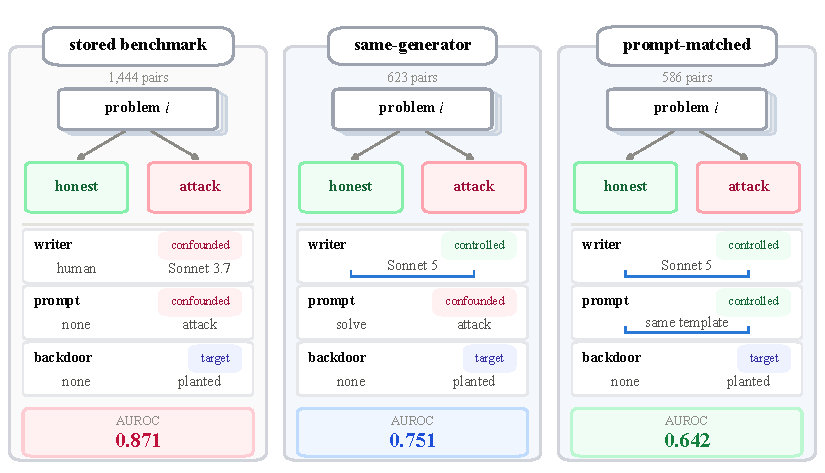
\includegraphics[width=\linewidth]{f4-constructions.pdf}
\caption{\textbf{How a stored pair is built, and how we rebuild it.} Each row is one property of
the pair: written once and tied, it is identical on the two sides; written twice, it differs. As
stored, the honest program is human-written and the backdoored one model-written, so the classes
differ in writer and in elicitation as well as in sabotage. We hold the writer constant, then the
prompt as well (the tinted columns), the two prompts being identical apart from the sentences that
ask for a flaw. The backdoor row never merges, and it is the only difference a monitor should
read. Under each construction is the same bag-of-words classifier's AUROC on it, on one scale from
chance to 1.0; every arm's $S$, $B'$ and $\rho$ are in Table~\ref{tab:gates}.}
\label{fig:constructions}
\end{figure}

The corpora we measure are built on that artifact. We use seven public corpora, whose
per-class provenance is the object of study. In the APPS family the honest class is human and
the attack class is one of ten named models. Six of the seven declare no licence
\cite{koran2026highquality, sinha2026controlarenacorpora}, so we report only aggregates and
redistribute no corpus.

Our headline protocol is one of the seven, the filtered, comment-stripped split
\cite{koran2026ensemble}: \splitTrain{} train problems (\splitTrainItems{} paired items) and
\splitTest{} test items (\splitAttack{} attack, \splitHonest{} honest), labelled by
\texttt{backdoor\_works}, reconstructed with the released harness code
\cite{jha2026decorrelation}. Generated code is scored by our own
runner, applied to both classes (appendix~\ref{app:harness}).

% =====================================================================================
\section{Results}
\label{sec:results}
% Budget: ~780 words. F1 is Table~\ref{tab:protocol-baseline} in the appendix; F3 is the
% one body float.
% =====================================================================================

Comment stripping works on comment count and code length, driving both to chance
(Table~\ref{tab:protocol-baseline}, appendix). Two floors on that same split do not move. A
monitor scoring at or below a floor has shown nothing beyond what the corpus leaks.
Bag-of-words reaches \tfidfKoran{} and a classifier that reads no code at all reaches
\nocodeCV{}, both far above their permutation nulls and above \tfidfKoranCount{} of the
\monN{} monitors ranked on that split (Figure~\ref{fig:monitors}; intervals, nulls and
paired-bootstrap counts in appendix~\ref{app:protocol}).

Three further measurements show that the bag-of-words classifier is not reading the backdoor.
Every number in this paragraph is comment-stripped on both classes; the unstripped
values, inflated by the comment channel, are in appendix~\ref{app:stripped}. The classifier
\emph{transfers across backdoor generators} at \transfer{} pairwise. Trained on one
attacker's backdoors it identifies another's, so it has learned a feature the attackers
share. It is also nearly as strong on \emph{inert} backdoors
(\pairInert{}) as on working ones (\pairWorking{}), where a detector of sabotage should
find the backdoors that never function much harder. And the residual carrier is stylistic.
\texttt{\_\_main\_\_} appears in 0.116 of attack samples against 0.000 of
honest ones, replicated on the train split (152 versus 1 of \splitTrain{}) and untouched by
the stripper. A token-level version of the test does not replicate here
(appendix~\ref{app:token}).

To test whether authorship is what the classifier reads, we hold the author constant and
measure how much separability survives. Under the identical pipeline the human-honest baseline is $B = \baselineB$ over
$n = \baselineBn{}$ pairs. Write $G$ for that same quantity when one model writes both classes.
Retained signal is $\rho = (G - 0.5)/(B - 0.5)$: $\rho = 1$ means holding authorship constant
changed nothing, $\rho = 0$ that nothing survived. We pre-registered $\rho \le \rhoCollapse{}$
as authorship and $\rho > \rhoContent{}$ as content, and fixed both bands before any arm ran.

% --- Gate S outcome, in three paragraphs plus Table~\ref{tab:gates} (notes/12 §1: the
%     single highest-value change of the cold review). EVERY row-level number now lives in
%     the table or its caption; the prose keeps the reading and the mechanism. Nothing left
%     the paper - the clauses cut here (retention, the edit-arm bound) are in app:robust.
One model writing both classes removes between a third and nine-tenths of the separability
(Table~\ref{tab:gates}). We report the \emph{independent} arm, in which the
attack class is written from the problem statement alone, so authorship changes and nothing else.
An \emph{edit} arm, shown its own honest solution, returns near-copies instead
(appendix~\ref{app:pairsim}). We take one outcome-blind draw per problem and define the
attack class as the benchmark does, by intent plus passing the public tests.
\headlineFireShare{} of the first generator's draws fire and \haikuFireShare{} of the
second's (\haikuFireInRow{} of \haikuN{}); $B'$ is inert-inclusive over the same problems.
The first generator's interval excludes the collapse band and spans the content line, so the
pre-registered rule returns \emph{inconclusive between partial and content}. The second
generator's lies inside the collapse band. Sample size does not explain the drop, since at
$n = \sameGenN{}$ the baseline $B$ under the identical pipeline is $\curveHeadline{} \pm
\curveHeadlineSd{}$. Two rows are
\emph{strict}: they keep only attacks that pass the tests \emph{and} fire on their trigger,
selected by the benchmark's own retry-and-keep. Only
\strictN{} pairs meet it,
so we read them through $\rho$ alone; they agree with the headline rows at low power.

\begin{table}[h]\centering\footnotesize
\setlength{\tabcolsep}{4pt}
\caption{\textbf{What is left when one model writes both classes.} $S$ is the
same-generator AUROC (5-fold, comments stripped) and $B'$ the stored-pair baseline on the
row's own problems; $\rho$, its bands and its intervals are as in the text and
appendix~\ref{app:robust}.}
\label{tab:gates}
\begin{tabular}{@{}l r l r l l@{}}
\toprule
Arm & $n$ & $S$ (95\% CI) & $B'$ & $\rho$ (95\% CI, joint) & band \\
\midrule
Sonnet 5, headline & \sameGenN{} & \sameGenS{} (\sameGenLo{}--\sameGenHi{})
  & \sameGenBprime{} & \sameGenRho{} (\sameGenRhoLo{}--\sameGenRhoHi{}) & partial--content \\
Haiku 4.5, headline & \haikuN{} & \haikuS{} (\haikuSLo{}--\haikuSHi{})
  & \haikuBprime{} & \haikuRho{} (\haikuRhoLo{}--\haikuRhoHi{}) & \textbf{collapse} \\
Sonnet 5, prompt-matched & \matchedN{} & \matchedS{} (\matchedLo{}--\matchedHi{})
  & \matchedBprime{} & \matchedRho{} (\matchedRhoLo{}--\matchedRhoHi{}) & \textbf{partial} \\
Sonnet 5, strict & \strictN{} & \strictS{} (\strictLo{}--\strictHi{})
  & \strictBprime{} & \strictRho{} (\strictRhoLo{}--\strictRhoHi{}) & partial--content \\
Sonnet 5, strict, matched & \matchedStrictN{} & \matchedStrictS{} (\matchedStrictLo{}--\matchedStrictHi{})
  & \matchedStrictBprime{} & \matchedStrictRho{} (\matchedStrictRhoLo{}--\matchedStrictRhoHi{}) & partial--content \\
\bottomrule
\end{tabular}
\end{table}

The attack prompt separates the two generators. On Sonnet 5 the surviving signal is
lexical, with length alone falling to \sameGenLen{} while TF-IDF holds, and it does not run
through the trigger. Masking numerals and comparison operators leaves $S$ unchanged;
only normalising identifiers moves it, to \sameGenSid{} ($\rho = \sameGenRhoId{}$). The top
attack-side features are \texttt{def main} (\defMainAttack{} of attack programs against
\defMainHonest{} of honest ones) and \texttt{data[}, which together are the program layout the
attack prompt elicits. Haiku 4.5 never adopts that layout. \texttt{def main} and
\texttt{sys.stdin} appear in no program of any of its three classes, which read input with
\texttt{input(} throughout (appendix~\ref{app:secondpass}). Holding the prompt constant as
well as the model therefore moves the two generators toward each other, to
$\rho = \matchedRho{}$ and $\rho = \haikuMatchedRho{}$. On Sonnet this removes most of what
is left. The two honest classes alone, with no attack on either side, already separate at
\promptOnly{}, so the prompt is carrying framing and no backdoor at all. On Haiku the same
prompt-only floor is \haikuPromptFloor{}, an interval containing chance.

Regenerating one class rather than both does not work. With an open-weight model writing the
honest class against the stored backdoors, separation is higher than the stored baseline, at
$\rho = \armOneRho{}$ (appendix~\ref{app:robust}): the original authorship gap has been
replaced by a new one between that model and the stored attacker.

The same inflation appears when the detector is an LLM monitor rather than a bag-of-words
classifier. We put a zero-shot monitor prompt to the model that wrote both classes. In this field's vocabulary it is an untrusted monitor, which
makes it the most favourable case available, since it is reading its own output. On the \emph{stored} pairs over the headline problems it scores
\monStoredHead{} and on the same-generator pairs \monitorS{}, a monitor-$\rho$ of
\monRhoHead{}, below the classifier's \sameGenRho{}. On the strict pairs it scores
\monStoredStrict{} and \monitorStrict{}, a monitor-$\rho$ of \monRhoStrict{} (intervals in
appendix~\ref{app:monitors}). A monitor that wrote neither class
returns the same two ratios: \monHaikuRhoHead{}, a bound at half missingness, and
\monHaikuRhoStrict{}. Our single-shot attacks fire given a pass at \fireGivenPassOurs{}
against the stored attacker's \fireGivenPassStored{}, which makes the stored attack class a
survivor set.

The split selects on a second property besides authorship. Labelling by
\texttt{backdoor\_works} defines the negative class at the problem level by \emph{attack
failure}; the criterion should be honesty. \inertShare{} of the test split's labelled
backdoors do not work (\inertSharePassing{} of those that pass the public tests), and a
problem whose backdoor fails contributes its human honest solution instead. The label is
fixed before any code is read. Attack problems also carry half as many test cases
(\testCasesAttack{} versus \testCasesHonest{}), and fewer tests make a backdoor easier
to hide, so difficulty and test count correlate with the label. That correlation produces the
content-blind \nocodeCV{}.

Removing the authorship gap does not remove every floor. In five settings where the same
three models write both classes, so no authorship confound is possible, the surviving floor
is structural: \bashFloor{} (\texttt{bash}, on its
null) to \agentdojoFloor{} (\texttt{agentdojo}) from character count alone
(Figure~\ref{fig:corpora}).

% =====================================================================================
\section{Limitations}
% Budget: three paragraphs. Disclosures owed by notes/05 are in the second.
% =====================================================================================

A high floor is evidence about a corpus; it does not settle results computed on that corpus.
Our floors show that the label is recoverable without reading a backdoor. They
say nothing about whether any monitor recovers it that way, and no number here corrects a
published monitor score.

The control arm is limited by the generator we had to substitute. The model that wrote the
stored backdoors, \texttt{claude-3-7-sonnet-thinking}, is retired, so
both same-generator classes come from a later model of the same lineage. It differs from the
stored attacker in backdoor style as well as in authorship, so every $\rho$ here, classifier or
monitor, bounds the content share of the separability instead of partitioning it. The arm is
not bit-reproducible, having run through a metered API that does not expose sampling
parameters, with thinking off although the stored attacker was a thinking model.

Our scope is narrow in three further ways. We measure one APPS-derived corpus family and five
agentic settings, and other stored-pair corpora are untested. Five of our seven corpora are one
user's repackaging of ControlArena releases, so our claims are scoped to those artifacts as
published. And two interpreter-era artifacts fall on opposite classes, so $B$ carries a small
execution-environment channel that the same-generator arm does not
(appendix~\ref{app:harness}).

% =====================================================================================
\section{Discussion}
% Prose, not a checklist. None of the five papers this paper is submitted alongside ends on a
% bulleted list: Feng closes with Discussion then a four-sentence Conclusion, Koran, Terekhov
% and Little each carry a Discussion. The checklist register came from kapoor2022leakage,
% which is meta-science rather than an empirical venue paper. The run-in \paragraph labels
% this section used to carry were cut with the rest of the body's: every join is now a
% transition sentence, so do not reintroduce them here or in sections 2-4.
% =====================================================================================

These results imply one rule for construction: one model should write both classes under one
prompt framing, and one harness should verify both. Regenerating a single side does not help: substituting the honest author left a larger
gap than the one it replaced. Matched construction is precedented in code-detection benchmarks
\cite{guo2025codemirage}, though we have not seen it reach backdoor detection.

The definition of the negative class needs the same treatment. Defining it through attack
failure ties the label to the attacker rather than to the code, and puts a content-blind classifier
above most monitors ranked on this split; dropping the failed problems removes it, as does
sampling that class independently of attack success. A
monitor number is in turn interpretable only against the floors of its own split, so a
partial-input and a bag-of-words floor belong beside it, each against a permutation null, with
the split, the metric and the preprocessing released alongside (ours are MIT,
appendix~\ref{app:release}).

Stored pairs remain the cheapest way to develop a monitor, and nothing here argues for
abandoning them, only that a score on one describes two authors until the construction rules
that reading out.

% =====================================================================================
\bibliographystyle{plainnat}
\bibliography{refs}

% =====================================================================================
%  APPENDIX - not counted against the four content pages.
% =====================================================================================
\appendix
% Appendix floats are numbered A1, A2, ... so the body's Table 1 / Figure 1 stay Table 1 /
% Figure 1. Before this the body referenced Tables 2 and 3 (both here) before Table 1.
\setcounter{table}{0}\renewcommand{\thetable}{A\arabic{table}}
\setcounter{figure}{0}\renewcommand{\thefigure}{A\arabic{figure}}
\section{Supplementary tables and figures}

\subsection{The schema}
Table~\ref{tab:schema} is the record schema of \texttt{RoganInglis/apps-control-arena}
\cite{inglis2025appscontrolarena}. The attack class carries \texttt{model} and
\texttt{source}, naming the system that produced each backdoor; the honest class carries no
such field, because there is no generator to name. The two APPS-backdoor corpora we use are
two views of this one artifact, since every problem in the filtered release
\cite{koran2026highquality} is also in \cite{inglis2025appscontrolarena}, byte-identical
except a re-validated \texttt{backdoor\_works}. Among the agentic corpora we exclude
AgentHarm, to avoid a conflict of interest.

% The sub-field list must WRAP - as a plain `l' column it overflowed the 5.5in text block
% and the rules ran off the page edge.
\begin{table}[h]\centering\footnotesize
\setlength{\tabcolsep}{4pt}
\caption{The confound is legible in the dataset schema, with no measurement at all.
The attack class records which model wrote it; the honest class has no generator field.
Verified against the shard schema of \texttt{RoganInglis/apps-control-arena}.}
\label{tab:schema}
\begin{tabular}{@{}l>{\raggedright\arraybackslash}p{0.80\linewidth}@{}}
\toprule
struct & sub-fields \\
\midrule
\texttt{solutions} & \texttt{code}, \texttt{compiles}, \texttt{passes\_tests} \\
\addlinespace
\texttt{backdoors} & \texttt{backdoor\_code}, \texttt{backdoor\_input},
                     \texttt{backdoor\_works}, \texttt{compiles},
                     \textbf{\texttt{model}}, \texttt{passes\_tests},
                     \textbf{\texttt{source}} \\
\bottomrule
\end{tabular}
\end{table}

% --- F3: the monitor comparison (the only body float) ----------------------------------
\begin{figure}[h]\centering
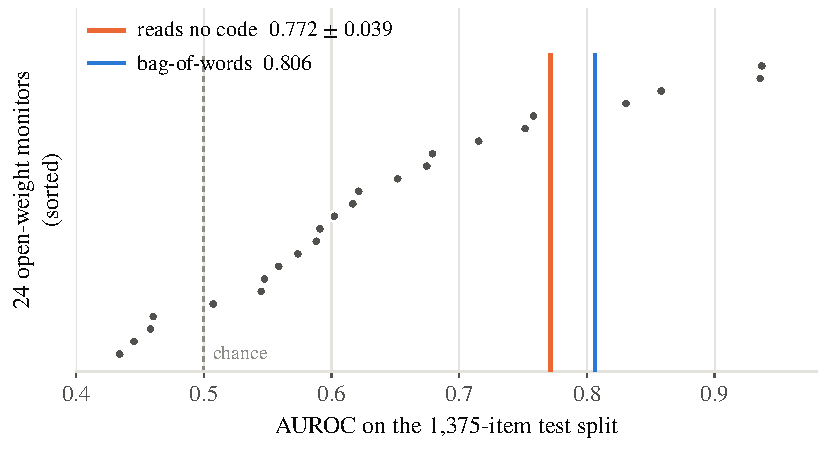
\includegraphics[width=0.64\linewidth]{f3-monitors-vs-floors.pdf}
\caption{\textbf{Two floors against the \monN{} open-weight monitors ranked on the same
split.} AUROC on the \splitTest{}-item test split (\splitAttack{} attack /
\splitHonest{} honest), comments stripped; monitor scores from the MIT-licensed release of
\cite{jha2026decorrelation}, median \monMedian{}, max \monMax{}. Both floors clear
\tfidfKoranCount{} of the \monN{}. \textbf{Two caveats.} (i)~The monitors are
zero-shot prompted while the bag-of-words classifier is \emph{trained} on the benchmark's own
paired train split. The comparison states what the corpus makes recoverable and does not
claim that bag-of-words is a better monitor.
(ii)~The no-code floor is cross-validated \emph{within} the test split; on one
held-out slice it is \nocodeHeldout{}, above \nocodeHeldoutCount{} of \monN{}
(appendix~\ref{app:protocol}).}
\label{fig:monitors}
\end{figure}

\subsection{The protocol $\times$ baseline table}
\label{app:protocol}
The no-code floor is cross-validated \emph{within} the test split because the released
train/val split is paired and therefore metadata-balanced; its permutation null shuffles
labels for fitting and scoring alike.
Table~\ref{tab:protocol-baseline} is the full measurement behind \S\ref{sec:results}. Rows
are not comparable across protocols; the preprocessing column says whether comments were
stripped before the baseline read the code. Pairwise accuracies are given to three decimals
because their resolution over 2,641 pairs is one pair. Intervals in \S\ref{sec:results} are
bootstraps over problems (\bootDraws{} draws) and nulls are \permReps{} label permutations;
the held-out no-code row is barely above its own null: \nocodeHeldout{}
(CI \nocodeHeldoutLo{}--\nocodeHeldoutHi{}) against a 95th percentile of
\nocodeHeldoutNull{}, $p = \nocodeHeldoutP{}$, above \nocodeHeldoutCount{} of the \monN{}
monitors by point estimate and \nocodeHeldoutPairedCount{} with a paired interval excluding
zero. The no-code claim therefore rests on the cross-validated protocol.
The two floors of \S\ref{sec:results} in full: bag-of-words reaches \tfidfKoran{} (95\% CI
\tfidfKoranLo{}--\tfidfKoranHi{} by bootstrap over problems; permutation null 95th percentile
\tfidfKoranNull{}, $\permP$), above \tfidfKoranCount{} of the \monN{} monitors by point
estimate and \tfidfKoranPairedCount{} with a paired-bootstrap interval excluding zero; the
no-code floor reaches \nocodeCV{} (CI \nocodeCVLo{}--\nocodeCVHi{} on the pooled out-of-fold
\nocodeCVPooled{}; null \nocodeCVNull{}, $\permP$), above \nocodeCVCount{} and
\nocodeCVPairedCount{} respectively.

% --- F1: generated by experiments/apps/figures.py; do not hand-edit -----------------
% F1 - generated by experiments/apps/figures.py, do not hand-edit
\begin{table}[h]\centering\footnotesize
\setlength{\tabcolsep}{4pt}
\caption{What the field's preprocessing leaves behind. Every row is measured under the protocol named in column one; rows are not comparable across protocols. \emph{Prep.} says whether comments were stripped before the baseline read the code; \emph{no code} means the baseline never reads the program. The comments-kept rows are inflated by the comment channel and are given for contrast, not as results. The matched rows are problem-disjoint and scored against the DSPy tutorial monitor; the transfer row runs Control Tax to the GPT-4-era set. Pairwise accuracies are given to three decimals, their resolution over the pair count.}
\label{tab:protocol-baseline}
\begin{tabular}{@{}>{\raggedright\arraybackslash}p{0.255\linewidth}>{\raggedright\arraybackslash}p{0.225\linewidth}r>{\raggedright\arraybackslash}p{0.090\linewidth}>{\raggedright\arraybackslash}p{0.170\linewidth}@{}}
\toprule
Protocol & Baseline & Value & Prep. & Against \\
\midrule
\multicolumn{5}{@{}l}{\emph{AUROC}} \\
Koran's exact split & TF-IDF word 1--2gram & 0.8063 & stripped & above 20 of 24 \\
\quad same & TF-IDF word 1--2gram & 0.8914 & kept & above 22 of 24 \\
\quad same, reads no code & difficulty $+$ \#tests $+$ $|q|$ & 0.7715 $\pm$ 0.0389 & no code & above 20 of 24 \\
\quad same, held-out slice & difficulty $+$ \#tests $+$ $|q|$ & 0.7163 & no code & above 18 of 24 \\
\quad same & code length only & 0.4726 & stripped & chance \\
\quad same & \#-count detector & 0.4983 & stripped & chance \\
\quad same & \#-count detector & 0.6957 & kept & --- \\
Raw artifact, problem level & all metadata & 0.8917 & no code & --- \\
\quad same & difficulty only & 0.6823 & no code & --- \\
\quad same & \texttt{solution\_passes\_tests} & 0.7881 & no code & --- \\
Matched pairs (P3) & all metadata & 0.5000 & no code & by construction \\
\addlinespace
\multicolumn{5}{@{}l}{\emph{Pairwise accuracy}} \\
DSPy matched pairs & TF-IDF word 1--2gram & 0.897 & stripped & monitor 0.69--0.81 \\
\quad working backdoors only & TF-IDF word 1--2gram & 0.935 & stripped & --- \\
\quad \textbf{inert} backdoors only & TF-IDF word 1--2gram & 0.879 & stripped & not sabotage \\
\quad transfer, cross-generator & TF-IDF word 1--2gram & 0.969 & stripped & --- \\
\quad all pairs, comments kept & TF-IDF word 1--2gram & 0.962 & kept & --- \\
\quad working, comments kept & TF-IDF word 1--2gram & 0.979 & kept & --- \\
\quad inert, comments kept & TF-IDF word 1--2gram & 0.955 & kept & --- \\
\quad transfer, comments kept & TF-IDF word 1--2gram & 0.994 & kept & --- \\
\quad same, raw artifact & code length only & 0.826 & kept & --- \\
\bottomrule
\end{tabular}
\end{table}


\subsection{Comment stripping on the matched-protocol numbers}
\label{app:stripped}
The matched-pair and transfer measurements were first made with comments in. Every value in
the authorship paragraph of \S\ref{sec:results} was re-measured with the same stripper
applied to both classes, over five problem-disjoint splits (each transfer row is one fixed
split). With comments kept the same quantities were transfer \transferKept{}, working
\pairWorkingKept{}, inert \pairInertKept{}, all pairs \pairAllKept{} and surface-feature
AUROC \surfaceSevenKept{}; stripped they are \transfer{}, \pairWorking{}, \pairInert{},
\pairAll{} and \surfaceSeven{}. Every one was inflated by the comment channel, which is
this paper's thesis applied to itself. The \texttt{\#}-presence marker, \hashPresAttack{}
against \hashPresHonest{} before stripping, closes to \hashPresAttackStripped{} against
\hashPresHonestStripped{} after and is dropped; \texttt{\_\_main\_\_} is unchanged. One
authorship leak survives the stripper because string literals are not comments: in the
comment-stripped train split an author byline (\texttt{Author :}) survives in
\bylineHonest{} of \splitTrain{} honest samples against \bylineAttack{} attack samples, and
a triple-quoted block in \tripleHonest{} against \tripleAttack{}. Both are far too rare to
drive \tfidfKoran{}, but both are a literal record of authorship.
Stripped, the matched-protocol TF-IDF AUROC is \tfidfMatched{}, beside $B = \baselineB$ and
the Koran-split \tfidfKoran{}, all three on stripped code. The other cross-generator
transfer rows, stripped, are \transferOthreeClaude{} (o3-mini to claude-3-7-sonnet, 82 test
pairs), \transferClaudeOthree{} (the reverse) and \transferOoneGemini{} (o1-mini to
gemini-2.0-flash).

\subsection{Pair similarity, and why the same-generator control needs two arms}
\label{app:pairsim}
An attack class built by editing its own honest solution changes pair similarity as well as
authorship (Table~\ref{tab:similarity}); the independent arm sits in the stored benchmark's
regime and if anything slightly further from it, so it cannot manufacture a low $S$ by
making the classes alike.

\begin{table}[h]\centering\footnotesize
\setlength{\tabcolsep}{5pt}
\caption{Character similarity of honest/attack pairs, comments stripped. The edit arm's
classes are near-copies; the independent arm reproduces the stored benchmark's regime, where
the two classes are largely independent programs. The last two columns are the share of pairs
above and below those similarities.}
\label{tab:similarity}
\begin{tabular}{@{}l r r r l@{}}
\toprule
Attack class & mean sim. & share $>0.95$ & share $<0.60$ & changes vs.\ the benchmark \\
\midrule
\textbf{stored benchmark} & \simStored{} & \simStoredHigh{} & \simStoredLow{} & the regime to match \\
\textbf{edit} (shown its own solution) & \simEdit{} & \simEditHigh{} & \simEditLow{} & authorship \emph{and} similarity \\
\textbf{independent} (problem only) & \simIndep{} & \simIndepHigh{} & \simIndepLow{} & authorship only \\
\bottomrule
\end{tabular}
\end{table}

\subsection{Robustness of the same-generator rows}
\label{app:robust}
At the strict rows' $n = \strictN{}$, $B$ under the identical pipeline is $\curveStrict{} \pm
\curveStrictSd{}$. Intervals in the same-generator paragraphs of \S\ref{sec:results} are bootstraps over problems,
resampling $S$ and $B'$ jointly for $\rho$; this replaced a $\pm2$ fold-sd rule before the
retry pool was read. Every $\rho$ point we quote is the ratio of the fold-mean AUROCs and every
joint interval beside it is the bootstrap of the pooled out-of-fold $\rho$, which is the same
quantity computed two ways: the pooled points are \strictRhoPooled{} (strict, the row whose interval
Table~\ref{tab:gates} quotes), \matchedRhoPooled{} (prompt-matched headline),
\matchedStrictRhoPooled{} (prompt-matched strict) and \haikuRhoPooled{} (the second generator). Five fold seeds move the strict row's $\rho$ over \strictRhoSeeds{}.
Retention does not produce the effect. Survivors and non-survivors separate at only
\survivorAuroc{}, and $S$ computed with non-firing attempts on the same problems is
\survivorSwapS{} against \survivorSwapSref{}. The edit arm bounds $S$ under near-copies
(similarity \editSim{}, Table~\ref{tab:similarity}): \editS{} over \editN{} pairs,
$\rho = \editRho{}$. In arm 1, where only the honest half was regenerated, $G = \armOneG{}$ against
$B' = \armOneBprime{}$ on that arm's $n = \armOneN{}$ eligible problems, and TF-IDF gains
\armOneTfidfDelta{} while the length carrier collapses to \armOneLenG{}. Our own attack
prompt halves our single-shot firing rate:
\trigPublicShare{} of our test-passing draws offer a public test input as the trigger, which
cannot diverge from the honest solution, and those fire \trigPublicFire{} against
\trigNovelFire{} for novel triggers; no stored working backdoor has such a trigger
(\trigStoredPublic{}). The rest is retry-and-keep.

\subsection{The prompt-matched arm under the masks, and the second generator}
\label{app:secondpass}
Under prompt matching the identifier mask, the only mask of \S\ref{sec:results} that moved
$S$, takes the headline row to \matchedSid{} ($\rho = \matchedRhoId{}$) where it takes the
original honest class on the same \matchedN{} problems to \matchedSidOrig{}, so identifier
normalisation and prompt matching remove largely the same thing. That masked row is the one that decides whether the residue is structure or naming, and under
prompt matching it is band-ambiguous: its joint interval, \matchedRhoIdLo{}--\matchedRhoIdHi{},
puts \matchedRhoIdCollapse{} of its mass in the collapse band. A character model
(3--5-grams, same classifier and folds) retains more than the word tokeniser, \matchedChar{}
($\rho = \matchedRhoChar{}$), so the drop is not an artefact of tokenisation. On the strict
pairs the matched row is $S = \matchedStrictS{}$ ($n = \matchedStrictN{}$,
$\rho = \matchedStrictRho{}$, \matchedStrictRhoLo{}--\matchedStrictRhoHi{}).
The second generator's pairs are more self-similar than the first's (\haikuPairSim{} mean
against \simIndep{}), so $S$ was recomputed inside similarity strata, where it stays
\haikuStrataS{} in every stratum, including the \haikuStrataLowSim{}-similarity stratum,
which is further from its honest class than the stored benchmark's own pairs, while $B'$
holds \haikuStrataBprime{}, so near-copies are not what buys the collapse. Its prompt-matched
rows move $S$ to \haikuSMatched{} ($\rho = \haikuMatchedRho{}$, $n = \haikuMatchedN{}$) and put
the prompt-only floor at \haikuPromptFloor{}, an interval containing chance. The mechanism is
visible in the programs. The layout vocabulary that the first generator's residue is made of,
\texttt{def main}, \texttt{sys.stdin} and \texttt{data[}, is present in \haikuDefMain{} of the
second generator's programs in \emph{all three} of its classes, which read standard input with
\texttt{input(} in \haikuInputPresent{} of programs on every side, so there is no layout
difference left for the classifier to read.

\subsection{The monitor rows, and what bounds the second monitor}
\label{app:monitors}
The monitor that wrote both classes scores \monitorS{} (\monitorSLo{}--\monitorSHi{}) on the
same-generator headline pairs, a monitor-$\rho$ of \monRhoHead{}
(\monRhoHeadLo{}--\monRhoHeadHi{}); on the strict pairs it scores \monitorStrict{}
(\monitorStrictLo{}--\monitorStrictHi{}), a monitor-$\rho$ of \monRhoStrict{}
(\monRhoStrictLo{}--\monRhoStrictHi{}).
The monitor that wrote neither class scores \monHaikuHead{} on the same-generator headline
pairs and \monHaikuStoredHead{} on the stored pairs over the same problems, \monHaikuStrict{}
and \monHaikuStoredStrict{} on the strict pairs. Its headline rows bound the value without
fixing it. A 512-token reply ceiling left \monHaikuMissHead{} same-generator replies unparseable,
and on the stored side the missing share differs by class (\monHaikuMissHonest{} honest
against \monHaikuMissAttack{} attack), a bias of unknown sign. Re-running the strict pairs
with a 1{,}024-token ceiling prices it: missingness falls to 2 of 198 and monitor-$\rho$ moves
from \monHaikuRhoStrict{} to \monHaikuRhoStrictMt{}, inside the bootstrap interval.
On the stored pairs both monitors beat the bag-of-words baseline over the same problems
(\(+0.09\) and \(+0.15\) for the first, \(+0.02\) and \(+0.09\) for the second):
Figure~\ref{fig:monitors}'s ranking states something about those monitors on that split and
does not claim that a bag of words beats a monitor here. Classifier and monitor are independent pair
by pair on the same-generator pairs ($\phi = \monitorClfPhi{}$), so the two are reading
different things.

\subsection{The two generators' funnel}
Both generators were run through the identical pipeline. Our honest draws pass the public
tests at \sonnetHonestPass{} and \haikuHonestPass{} of 1{,}444 problems; the second
generator's attack draws pass at \haikuAttackPass{} of 1{,}444 and \haikuUsable{} of those
fire, below the 50-pair minimum \texttt{gate\_s\_samegen.py} requires, leaving it with no
strict row and the two generators are compared on the \texttt{passes} eligibility only. The two
compared rows differ in inertness. \haikuFireInRow{} of the \haikuN{} attacks in the
second generator's row fire (\haikuInert{} inert) against \relFireFirst{} of \sameGenN{}
(\headlineInert{}), the other \haikuUsableOutside{} of its firing draws sitting on problems where
its own honest program failed the tests and which the control therefore drops. The
single-shot firing rate belongs to the protocol and not to either model, since
\trigPublicShare{} of test-passing draws offer a public test input as their trigger.

\subsection{The five same-generator agentic settings}
Figure~\ref{fig:corpora} shows each setting's content-blind floor against its own
permutation null.

\begin{figure}[h]\centering
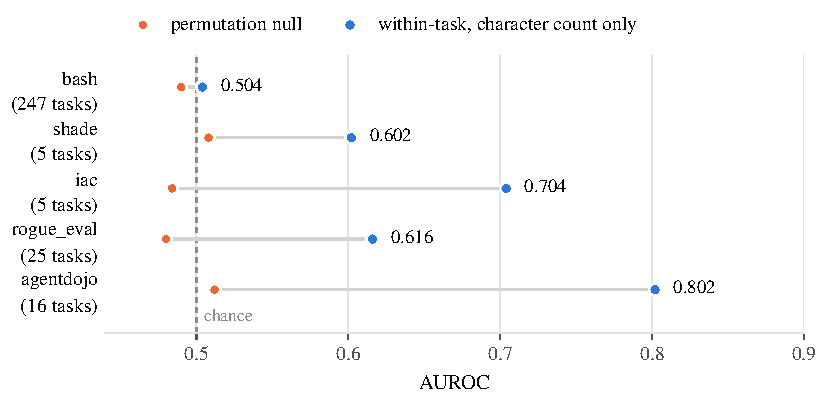
\includegraphics[width=0.86\linewidth]{f2-corpus-floors.pdf}
\caption{\textbf{The structural floor in five same-generator agentic settings.} Each
setting's content-blind classifier (six count features, no content read) scored
\emph{within task} against its own permutation null. No authorship confound is possible
here: claude-sonnet-4, gemini-2.5-pro and gpt-5 write both classes in all five.
\texttt{bash} sits on its null at \bashFloor{}; \texttt{agentdojo} reaches
\agentdojoFloor{} from character count alone. \textbf{The task-group count beside each
setting matters:} \texttt{shade} and \texttt{iac} average over five task groups each while
\texttt{bash} averages over 247, so these floors are not equally well determined. We report
the within-task column because our own pooled numbers partly broke on task composition,
and we broke them ourselves. The permutation nulls shown were computed with a pooled
estimator rather than the folded within-task statistic; they bound the chance level but
are not a like-for-like null for each dot. These corpora declare no licence; we
redistribute nothing and report aggregates only.}
\label{fig:corpora}
\end{figure}

\subsection{The release}
\label{app:release}
The supplementary bundle holds the same-generator split (\relHonest{} honest programs,
\relEdit{} edit-arm and \relIndep{} independent-arm attack programs written by one model,
plus every one of the \relRetryDraws{} draws of the independent arm's retry pool), both
eligibility rules as pair lists under an outcome-blind selection (\relPassFirst{} passing
and \relFireFirst{} firing independent-arm pairs) and under the benchmark's own survivor
selection (\relPassBest{} and \relFireBest{}, or \relFireBestCrash{} counting a crash on
the trigger as firing), the \relScripts{} scripts behind the measurements (generation for
both generators, the test harness, the trigger verifier, the selection rules, the prompt-matched
arm, the monitor rows and each remaining measurement script), a dataset card, and a manifest of
row counts and checksums. The licence, MIT, is a file inside the bundle and
covers the data and the scripts alike.

\subsection{The test harness and the pass flag}
\label{app:harness}
The same-generator arm requires executing generated code, so we built a runner that feeds each shipped
input case to a solution under per-case timeouts and address-space limits. It agrees with
the artifact's own \texttt{solution\_passes\_tests} on \harnessAgreement{} of the analysis
pool, and is strictly conservative there, never crediting a solution the artifact rejects
(\harnessFailWePass{} such cases). We use \emph{our own} flag for both classes, because a checker stricter on one class than
the other would manufacture exactly the artifact this paper documents. We do not length-match either class; the untrusted model chooses its own
trajectory length. The headline does not depend on that choice. Under the artifact's flag
$B = \baselineB$ at $n = \baselineBn{}$, under ours $B = \baselineBownflag{}$ at
$n = \baselineBownflagN{}$, within one standard deviation of each other. The monitor
scores in Figure~\ref{fig:monitors} are \texttt{runs/x0/monitor-summary.json} from the MIT
release of that harness \cite{jha2026decorrelation}, used under its notice. Two interpreter-era artifacts in the upstream solutions fall on opposite classes: a
\texttt{stdin} without \texttt{.buffer}, fixed, and \texttt{fractions.gcd}, removed in
Python~3.9, not fixable. $B$ is exposed to them; the same-generator arm, whose code we
generated and ran ourselves, is immune.

\subsection{The token test, run and failed}
\label{app:token}
We attempted to confirm a reported token-level mechanism \cite{orel2026aicd} in our setting and
it does not replicate. Separation is \tokenSep{}, the wrong sign, at permutation
$p = \tokenP{}$. The reason is register. Their human class is general-purpose repository
code, whereas \emph{both} of our classes are competitive-programming code, so an identifier
axis that separates general human code from model code does not separate these two
populations. Only 8 of their 10 canonical tokens are in our vocabulary, so the test is
underpowered; but an underpowered true effect would still carry the right sign, and this one
does not. We report it because a reader who knows that work may run exactly
this test.

\subsection{A third channel, noted but not developed here}
In the same five agentic settings a fifteen-word regular expression over the untrusted
policy's own scratchpad reaches \cotLow{}--\cotHigh{}, because prompted attack policies
restate their side task in the reasoning the monitor is given. We note this only to bound
the claim. The instrument is not ours, and the work it comes from \cite{little2026length}
validates it against an LLM judge and a length-matched null; we defer to that treatment.

\end{document}
